
    In this section we outline the estimated impact of MW changes on rent and house prices. We start by showing the results of our event-study specification with one event per zipcode. As discussed extensively in section \autoref{sec:empirical_strategy}, this model suffers from underidentification issues. We show several ways in which we address those. Later, we present results for the first difference specification, which we deem more reliable. Finally, we discuss the magnitude of the estimates.


\subsection{Event-study specification}\label{subsec:results/event-study}

    In this subsection, we present estimation results using median rents per square foot as our main dependent variable. In particular, we focus on the median rent per square foot for single family houses and condos (SFCC) as this is the most populated time series in the Zillow rent data. We show the robustness of our results by using alternative rent variables in the appendix. 
    %[ADD RESULTS FOR OTHER PSQFT RENT VARS TO THE APPENDIX]
    We also balance the panel and use zipcodes with valid rents data as of June 2015 only. This is to address concerns of changing composition of the sample.
    
    Figure \ref{fig:event_study_main} show estimations of the ``last event'' specification discussed in section \ref{sec:empirical_strategy}. As we discussed below, our preferred results consist of panels (e) and (f). We will go through the plots one by one. 
    
    The first row shows results of the specification in equation \eqref{eq:last-event-study}.
    
    The second row shows results of model \eqref{eq:last-event-study-countyFE}.
    
    The third row shows results of model \eqref{eq:last-event-study-control}.
    
    \begin{figure}[h!] \centering
        \caption{Dynamics around selected minimum wage events}
        \label{fig:event_study_main}
        \begin{subfigure}{0.5\textwidth} \centering
            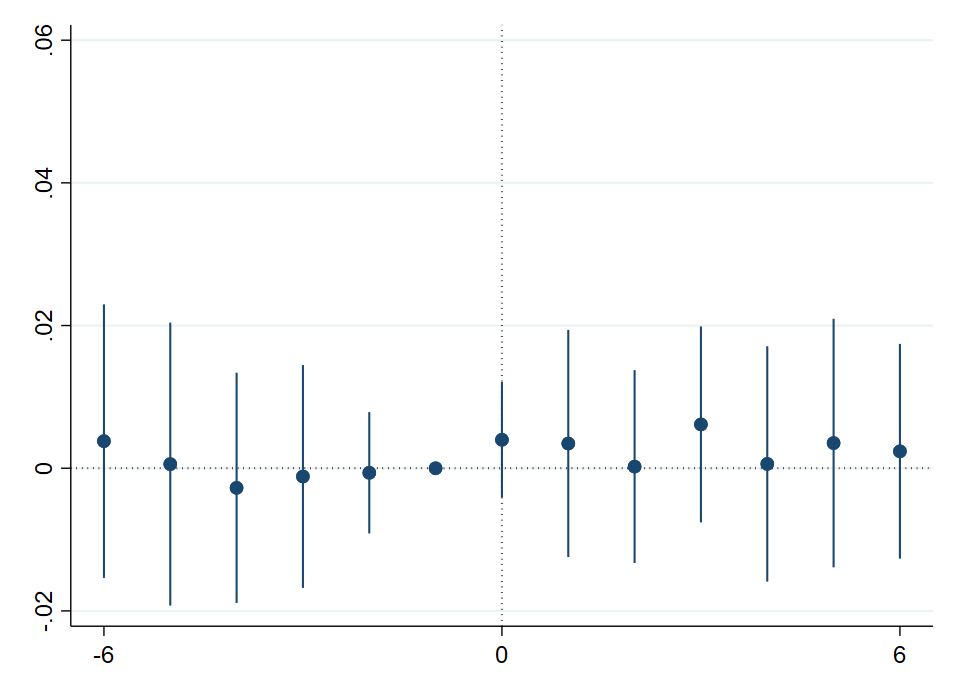
\includegraphics[width=0.95\linewidth]{analysis/event_study_exploration/output/last_rentpsqft_sfcc_zfe_w6.png}
            \caption{Naive TWFE with treated units only} \label{fig:event_study_treated}
        \end{subfigure}%
        \begin{subfigure}{0.5\textwidth} \centering
            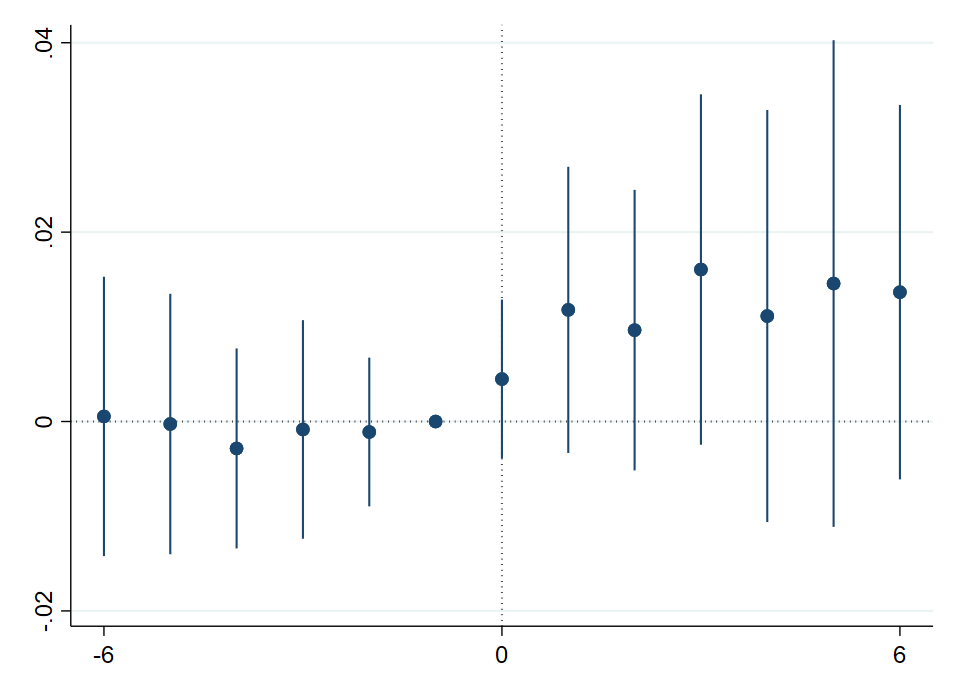
\includegraphics[width=0.95\linewidth]{analysis/event_study_exploration/output/last_rentpsqft_sfcc_zfe_w6_county-trend.png}
            \caption{Naive TWFE and county-specific trend} \label{fig:event_study_treated_county-trends}
        \end{subfigure}\\
        \begin{subfigure}{0.5\textwidth} \centering
            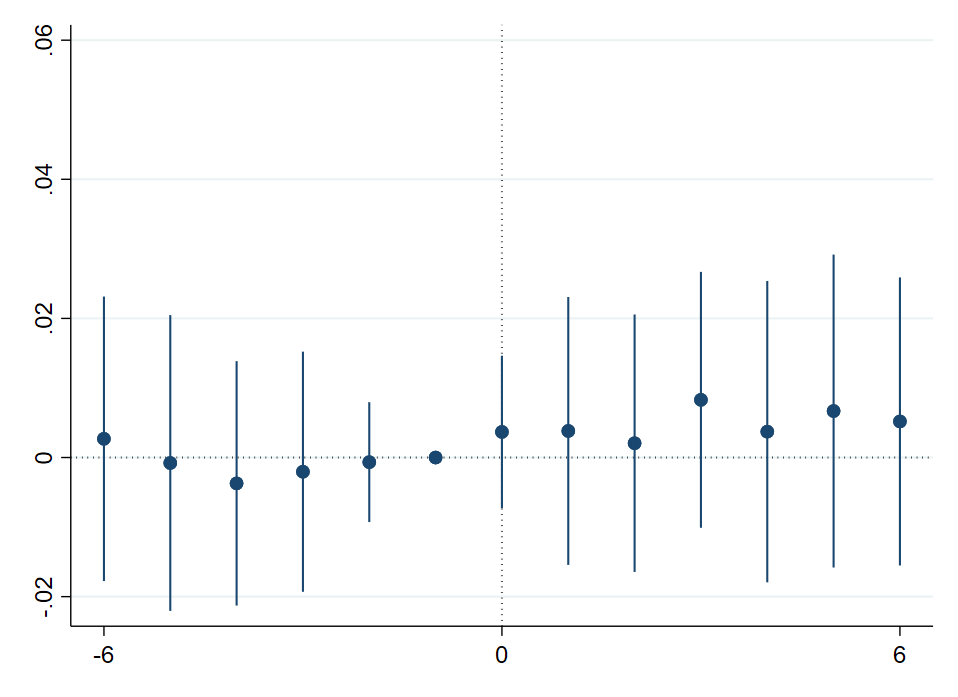
\includegraphics[width=0.95\linewidth]{analysis/event_study_exploration/output/last_rentpsqft_sfcc_cfe_w6.png}
            \caption{Replacing zipcode for county FE} \label{fig:event_study_countyFE_treated}
        \end{subfigure}%
        \begin{subfigure}{0.5\textwidth} \centering
            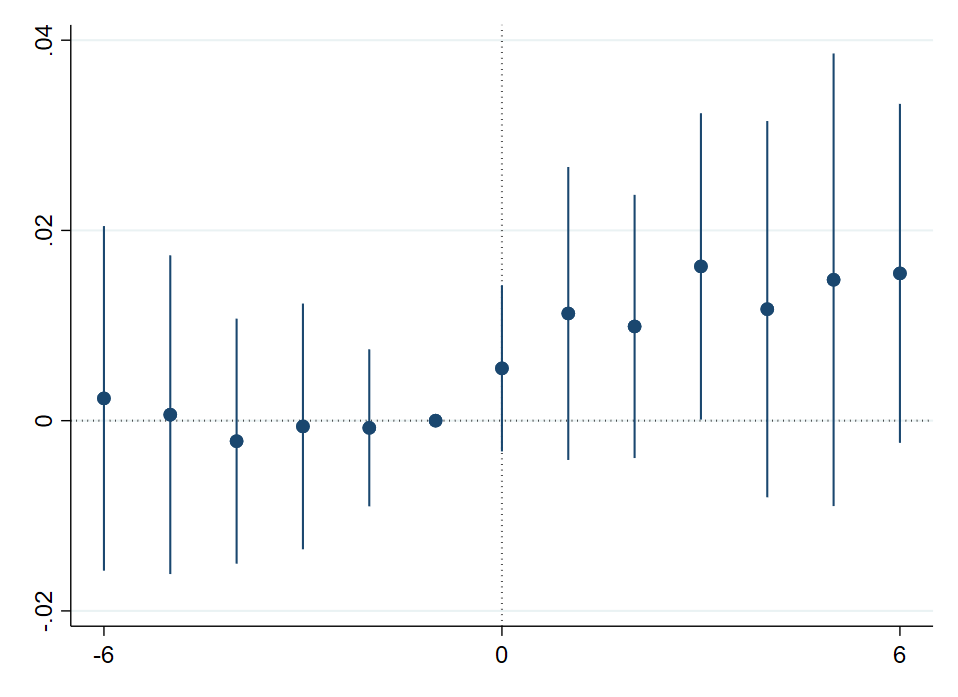
\includegraphics[width=0.95\linewidth]{analysis/event_study_exploration/output/last_rentpsqft_sfcc_cfe_w6_county-trend.png}
            \caption{\begin{tabular}{c} Replacing zipcode with county FE \\ and county-specific trend \end{tabular}} \label{fig:event_study_countyFE_treated_county-trends}
        \end{subfigure}\\
        \begin{subfigure}{0.5\textwidth} \centering
            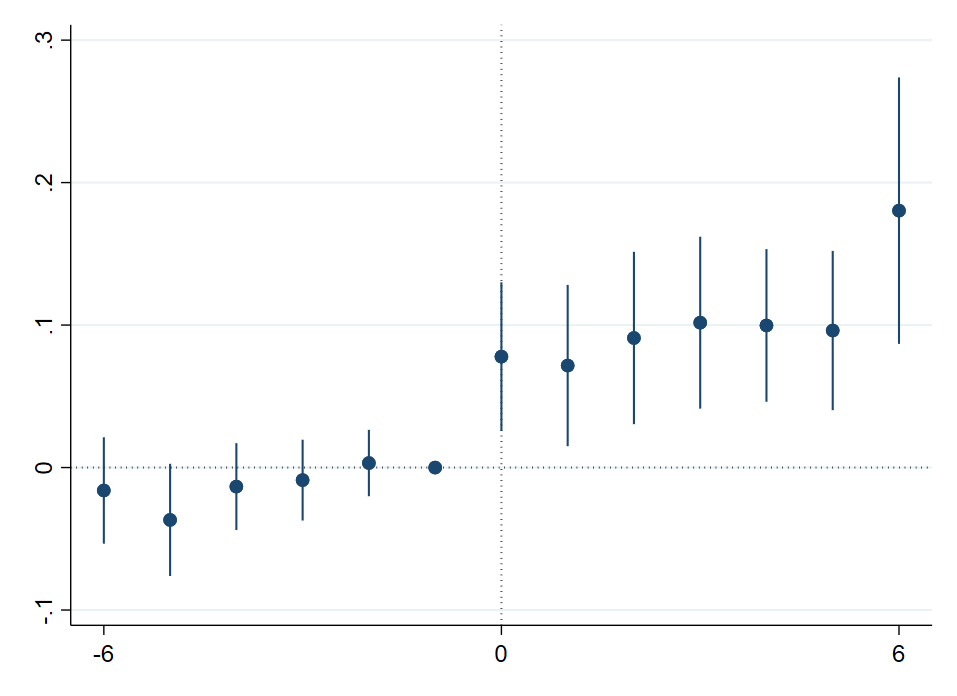
\includegraphics[width=0.95\linewidth]{analysis/event_study/output/last_rentpsqft_sfcc_w6.png}
            \caption{Naive TWFE with untreated units} \label{fig:event_study_all}
        \end{subfigure}%
        \begin{subfigure}{0.5\textwidth} \centering
            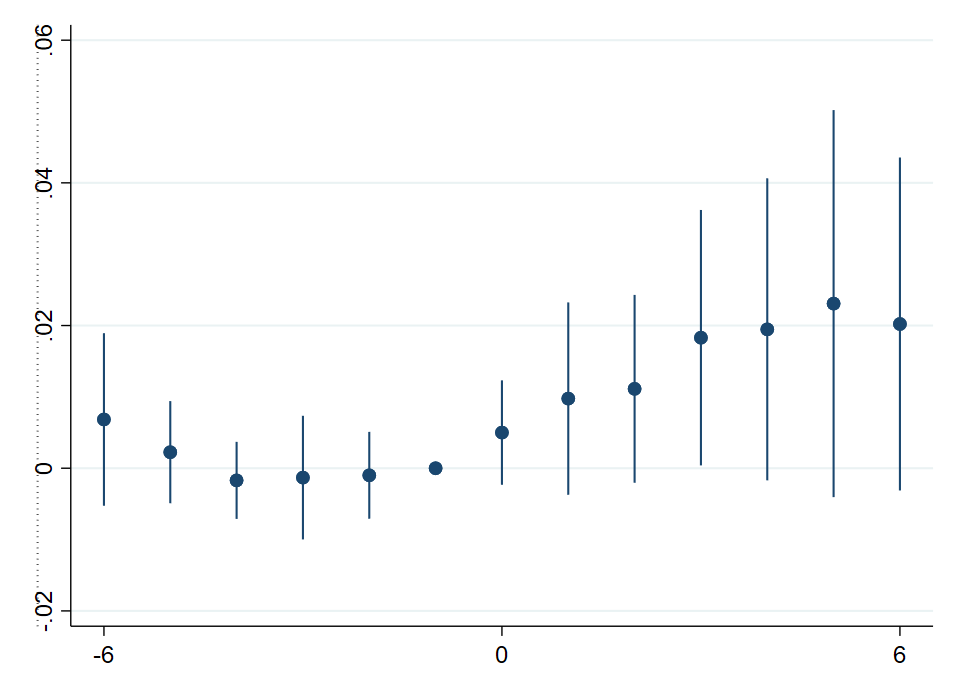
\includegraphics[width=0.95\linewidth]{analysis/event_study/output/last_rentpsqft_sfccw6_county-trend.png} \label{fig:event_study_all_county-trends}
            \caption{\begin{tabular}{c} Naive TWFE with untreated units \\ and county-specific trend \end{tabular}}
        \end{subfigure}\\
        \begin{minipage}{.95\textwidth} \footnotesize
			\vspace{2mm} 
			\textit{Notes}: Results from fitting the ``last event'' event study in different samples and with changing controls. All of the results select the last minimum wage event per zipcode, based on the requirement that the increase was of at least \$0.5 and that it took place before June 2019 (so that every event has at least 6 months after it). Furthermore, all models: use median rent per square foot of the SFCC category, and control for calendar time fixed effects (FE) and dummies for different categories of the cumulative sum of unused MW events. Each row is a different specification, with the panel on the right adding as controls county-specific linear and quadratic trend. Panels (a) and (b) fit the under-identified model using zipcode FE excluding never treated units (equation \ref{eq:last-event-study}), $N = 46,119$. Panels (c) and (d) use FE at the level of the county instead of zipcode, and keeps the sample of never treated units only (equation \ref{eq:last-event-study-countyFE}), $N = 46,119$. Panel (e) and (f) use zipcode FE and add control units (equation \ref{eq:last-event-study-control}), $N = 113,071$.
		\end{minipage}
    \end{figure}
    
    The causal claim on these results relies on the assumptions of no pre-trends. Indeed, all estimations show a rather flat and not statistically significant pre-trend %followed by a immediate impact of around ten cents on rent that remains stable in the following months.
    
    
    
    Second, we check the robustness of this result by changing the prominence of the MW changes. Specifically, In \ref{appfig:event_size_sensitivity} we use MW changes that comply to our sample criterion (explained in section 2) and are of at least \$0.25 and of at least \$0.75 instead of \$0.5.
    
    
    % TRY COUNTY-QUARTER SPECIFICATION
    
\subsection{Panel difference-in-differences specifications}\label{subsec:results/first-differences}

    \subsubsection{Baseline results}
    
    In this section we present the results from models based on section 4.2. Table XXX shows results from the static model in first differences. Column 1 reports results only including two way fixed effects. Column 2 adds a zipcode-specific linear trend, and column 3 a zipcode specific quadratic trend. 
    
    \begin{table}[h!] \centering
        \caption{Static model}
        \label{tab:fd_table}
        \scalebox{0.85}{
        {
\def\sym#1{\ifmmode^{#1}\else\(^{#1}\)\fi}
\begin{tabular}{l*{3}{c}}
\hline\hline
          &\multicolumn{1}{c}{(1)}&\multicolumn{1}{c}{(2)}&\multicolumn{1}{c}{(3)}\\
          &\multicolumn{1}{c}{D.ln\_med\_rent\_psqft}&\multicolumn{1}{c}{D.ln\_med\_rent\_psqft}&\multicolumn{1}{c}{D.ln\_med\_rent\_psqft}\\
\hline
D.ln\_mw   &   0.0257\sym{*}  &   0.0253\sym{**} &   0.0250\sym{**} \\
          & (0.0128)         & (0.0121)         & (0.0117)         \\
\hline
Zipcode-specifc linear trend&       No         &      Yes         &      Yes         \\
Zipcode-specific linear and square trend&       No         &       No         &      Yes         \\
R-squared &                  &                  &                  \\
Observations&    0.022         &    0.023         &    0.026         \\
N         &   113363         &   113363         &   113363         \\
\hline\hline
\end{tabular}
}
}
        \begin{minipage}{.95\textwidth} \footnotesize
			\vspace{3mm} 
			\textit{Notes}: Result
		\end{minipage}
    \end{table}
    
    
    In all cases the effects is significant, stable and a 10\% change in the MW implies around a 0.25\% increase in the rent per square foot. 
    
    Next, in Table XXX we show results from a model with 5 leads and lags of the logarithm of the MW. Again, Column 1 reports results of a specification with two way fixed effects. Column 2 adds a zipcode-specific linear trend, and column 3 a zipcode specific quadratic trend. 
    
    \begin{table}[h!] \centering
        \caption{Dynamic model}
        \label{tab:fd_table}
        \scalebox{0.85}{
        {
\def\sym#1{\ifmmode^{#1}\else\(^{#1}\)\fi}
\begin{tabular}{l*{5}{c}}
\hline\hline
          &\multicolumn{1}{c}{(1)}         &\multicolumn{1}{c}{(2)}         &\multicolumn{1}{c}{(3)}         &\multicolumn{1}{c}{(4)}         &\multicolumn{1}{c}{(5)}         \\
\hline
$\Delta \ln \underline{w}_{ic,t-5}$&  -0.0148         &  -0.0144         &  -0.0144         &  -0.0146         &  -0.0144         \\
          & (0.0090)         & (0.0089)         & (0.0089)         & (0.0090)         & (0.0089)         \\
[1em]
$\Delta \ln \underline{w}_{ic,t-4}$&  -0.0024         &  -0.0019         &  -0.0020         &  -0.0022         &  -0.0019         \\
          & (0.0116)         & (0.0116)         & (0.0115)         & (0.0116)         & (0.0115)         \\
[1em]
$\Delta \ln \underline{w}_{ic,t-3}$&   0.0011         &   0.0005         &   0.0007         &   0.0004         &  -0.0002         \\
          & (0.0092)         & (0.0094)         & (0.0092)         & (0.0091)         & (0.0092)         \\
[1em]
$\Delta \ln \underline{w}_{ic,t-2}$&   0.0060         &   0.0063         &   0.0062         &   0.0060         &   0.0064         \\
          & (0.0116)         & (0.0118)         & (0.0116)         & (0.0115)         & (0.0117)         \\
[1em]
$\Delta \ln \underline{w}_{ic,t-1}$&  -0.0002         &  -0.0004         &  -0.0005         &   0.0000         &  -0.0005         \\
          & (0.0123)         & (0.0123)         & (0.0124)         & (0.0122)         & (0.0123)         \\
[1em]
$\Delta \ln \underline{w}_{ic,t}$&   0.0271\sym{**} &   0.0257\sym{**} &   0.0259\sym{**} &   0.0269\sym{**} &   0.0259\sym{**} \\
          & (0.0126)         & (0.0123)         & (0.0124)         & (0.0126)         & (0.0124)         \\
[1em]
$\Delta \ln \underline{w}_{ic,t+1}$&   0.0136\sym{*}  &   0.0146\sym{**} &   0.0142\sym{*}  &   0.0135\sym{*}  &   0.0146\sym{*}  \\
          & (0.0072)         & (0.0072)         & (0.0072)         & (0.0072)         & (0.0072)         \\
[1em]
$\Delta \ln \underline{w}_{ic,t+2}$&  -0.0070         &  -0.0066         &  -0.0064         &  -0.0068         &  -0.0064         \\
          & (0.0133)         & (0.0133)         & (0.0132)         & (0.0133)         & (0.0132)         \\
[1em]
$\Delta \ln \underline{w}_{ic,t+3}$&   0.0036         &   0.0045         &   0.0047         &   0.0031         &   0.0040         \\
          & (0.0081)         & (0.0078)         & (0.0078)         & (0.0079)         & (0.0077)         \\
[1em]
$\Delta \ln \underline{w}_{ic,t+4}$&   0.0108         &   0.0093         &   0.0104         &   0.0107         &   0.0096         \\
          & (0.0069)         & (0.0066)         & (0.0064)         & (0.0069)         & (0.0065)         \\
[1em]
$\Delta \ln \underline{w}_{ic,t+5}$&   0.0086         &   0.0095         &   0.0099         &   0.0088         &   0.0099         \\
          & (0.0069)         & (0.0065)         & (0.0065)         & (0.0067)         & (0.0065)         \\
\hline
\vspace{-2mm}&                  &                  &                  &                  &                  \\
Cumulative effect&    0.057         &0.057\sym{*}         &0.059\sym{*}         &    0.056         &0.058\sym{*}         \\
          &  (0.035)         &  (0.034)         &  (0.034)         &  (0.034)         &  (0.034)         \\
\hline    &                  &                  &                  &                  &                  \\
P-value no pretrends&    0.568         &    0.612         &    0.599         &    0.594         &    0.629         \\
Wage controls&       No         &      Yes         &       No         &       No         &      Yes         \\
Employment controls&       No         &       No         &      Yes         &       No         &      Yes         \\
Establishment-count controls&       No         &       No         &       No         &      Yes         &      Yes         \\
R-squared &    0.022         &    0.022         &    0.022         &    0.022         &    0.022         \\
Observations&  106,446         &  105,463         &  105,463         &  106,160         &  105,463         \\
\hline\hline
\end{tabular}
}
}
        \begin{minipage}{.95\textwidth} \footnotesize
			\vspace{3mm} 
			\textit{Notes}: Result
		\end{minipage}
    \end{table}
    
    We also report the p-value of a test of $\beta_{-5} = \beta_{-4} = ... = \beta_{-1} = 0$. In all 3 cases we comfortably fail to reject that all leads are equal to 0 at the 95\% level. This is evidence that the pre-existing time paths of rent per square foot in zipcodes where the MW changed is not significantly different that the one for zipcodes in which the change didn't happened on that same time period. Given this, we estimate a model in which we assume all the leads are 0, and we include 5 lags of the logarithm of the MW (we call this model the distributed lags model). The coefficients from this estimation, plus the ones from the specification including 5 leads and lags are plotted in Figure XXX along with the path of effects implied by the static and distributed lags model. 
    
    \begin{figure}[h!] \centering
        \caption{Implied effect of different models}
        \label{fig:fd_models}
        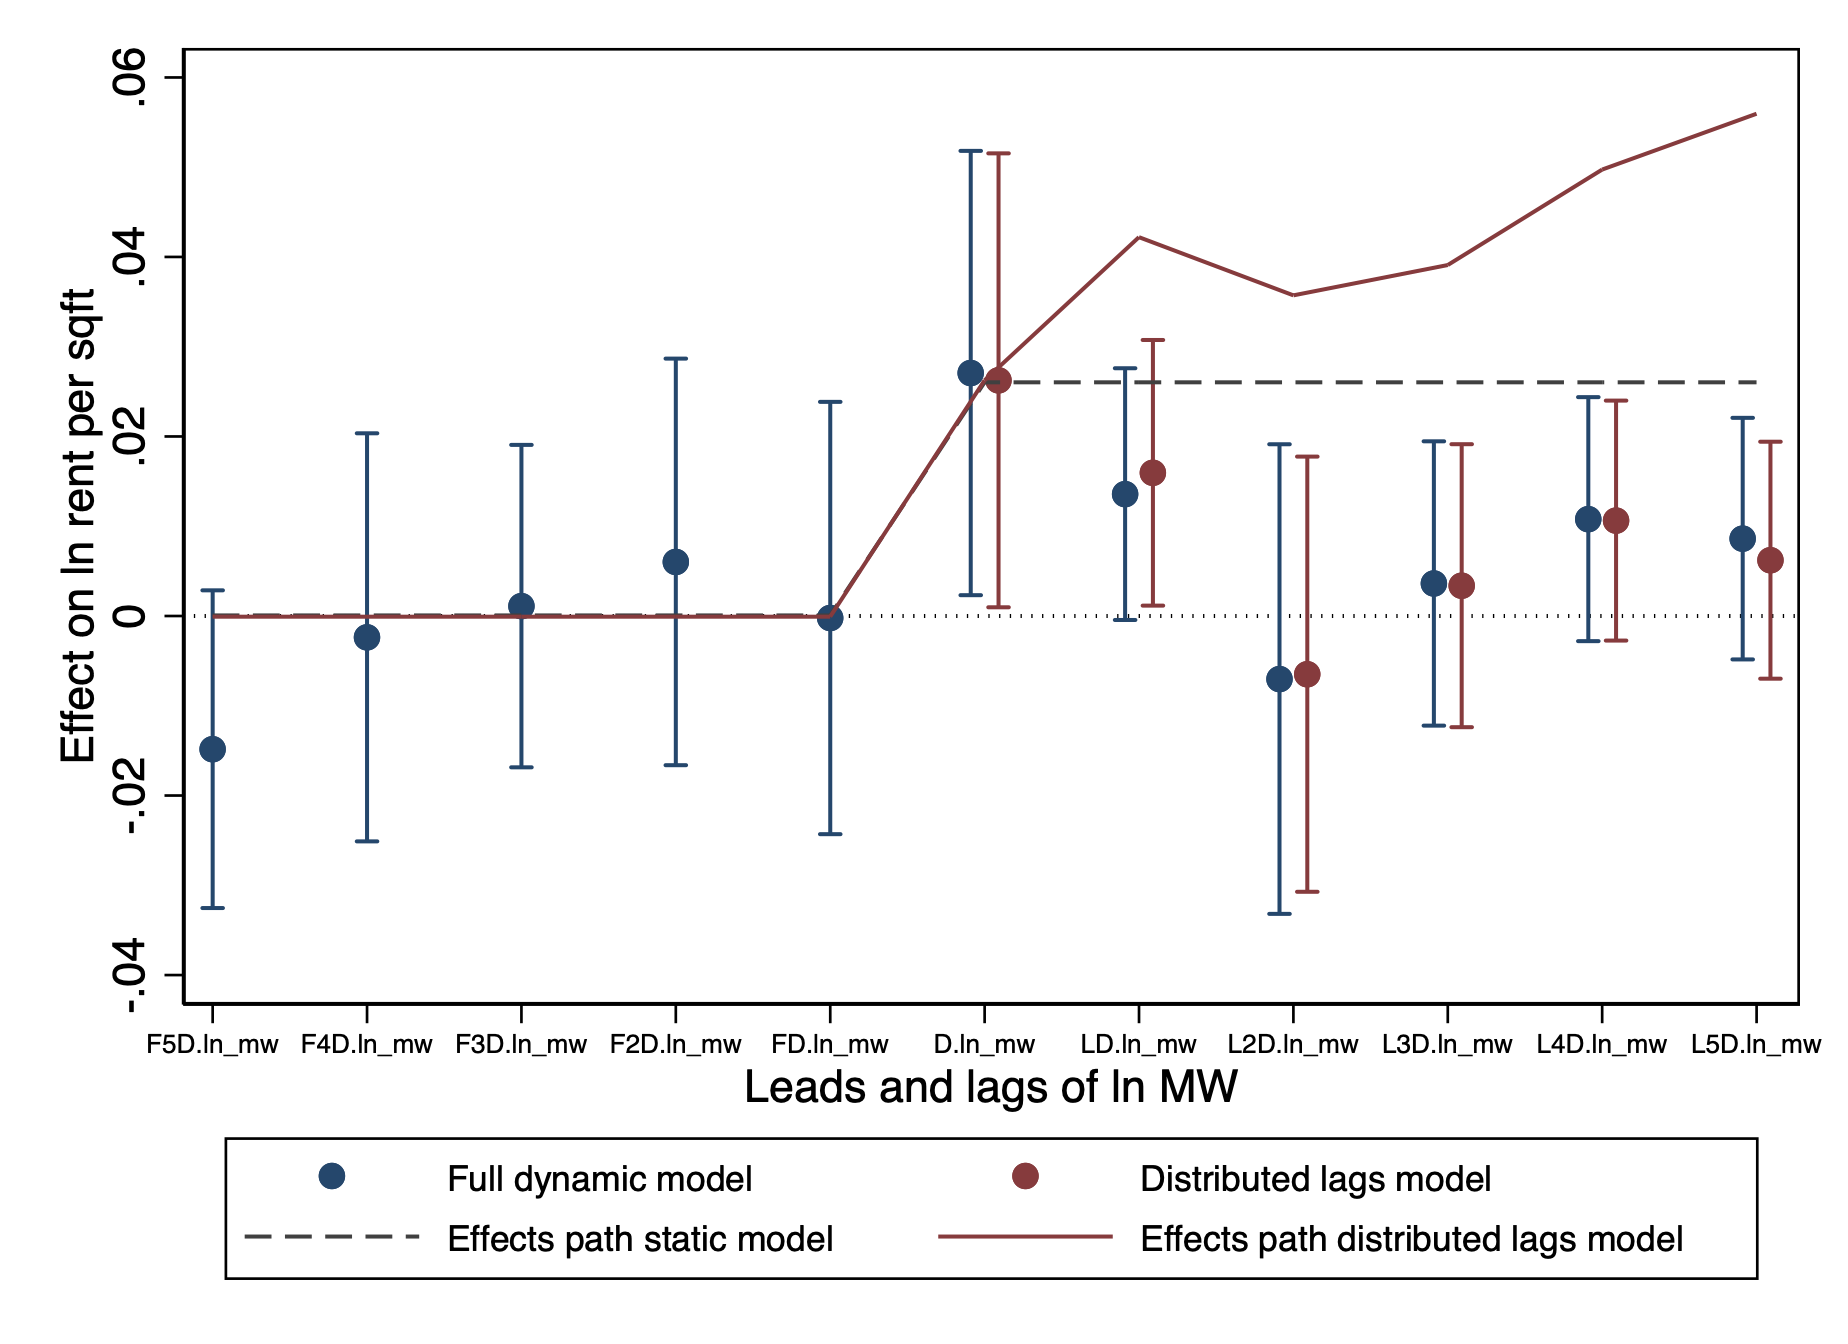
\includegraphics[width=0.75\linewidth]{analysis/first_differences/output/fd_models.png}
        \begin{minipage}{.95\textwidth} \footnotesize
			\vspace{2mm} 
			\textit{Notes}: Results 
		\end{minipage}
    \end{figure}
    
    We can see that there is no evidence of pretrends, and that the effects implied by the dynamic models are slightly larger than the ones implied by the static one.  
    
    
    \subsubsection{Heterogeneity by income}
    
    In order to explore whether the effects of MW on rents are mainly driven by "minimum wager" zipcodes we divide the set of zipcodes into median household income quintiles from the 2010 census and we run the following model:
    
    \begin{equation}\label{eq:diff_main}
            \Delta \tilde{y}_{it} = \theta_t + \gamma_i + \sum_{q=1}^5 \beta_q \mathds{1}\{i\in q\} \Delta \tilde{MW}_{it}+ \Delta \epsilon_{it}
    \end{equation}
    
    Were $q$ indexes median household income quintiles, and $\mathds{1}\{i\in q\}$ is 1 if zipcode $i$ belongs to the $q$th quintile of median household income. 
    
    The results are displayed in the following figure. As expected, zipcodes in the lower quintile have an effect that significant and much larger in magnitude the baseline effect on the full sample of zipcodes.
    
    Further heterogeneity in Appendix Figure \ref{appfig:fd_heterogeneity_appendix}.
    
    \begin{figure}[h!] \centering
        \caption{Heterogeneity of effect across zipcode median income quintiles}
        \label{fig:fd_heterogeneity_income}
        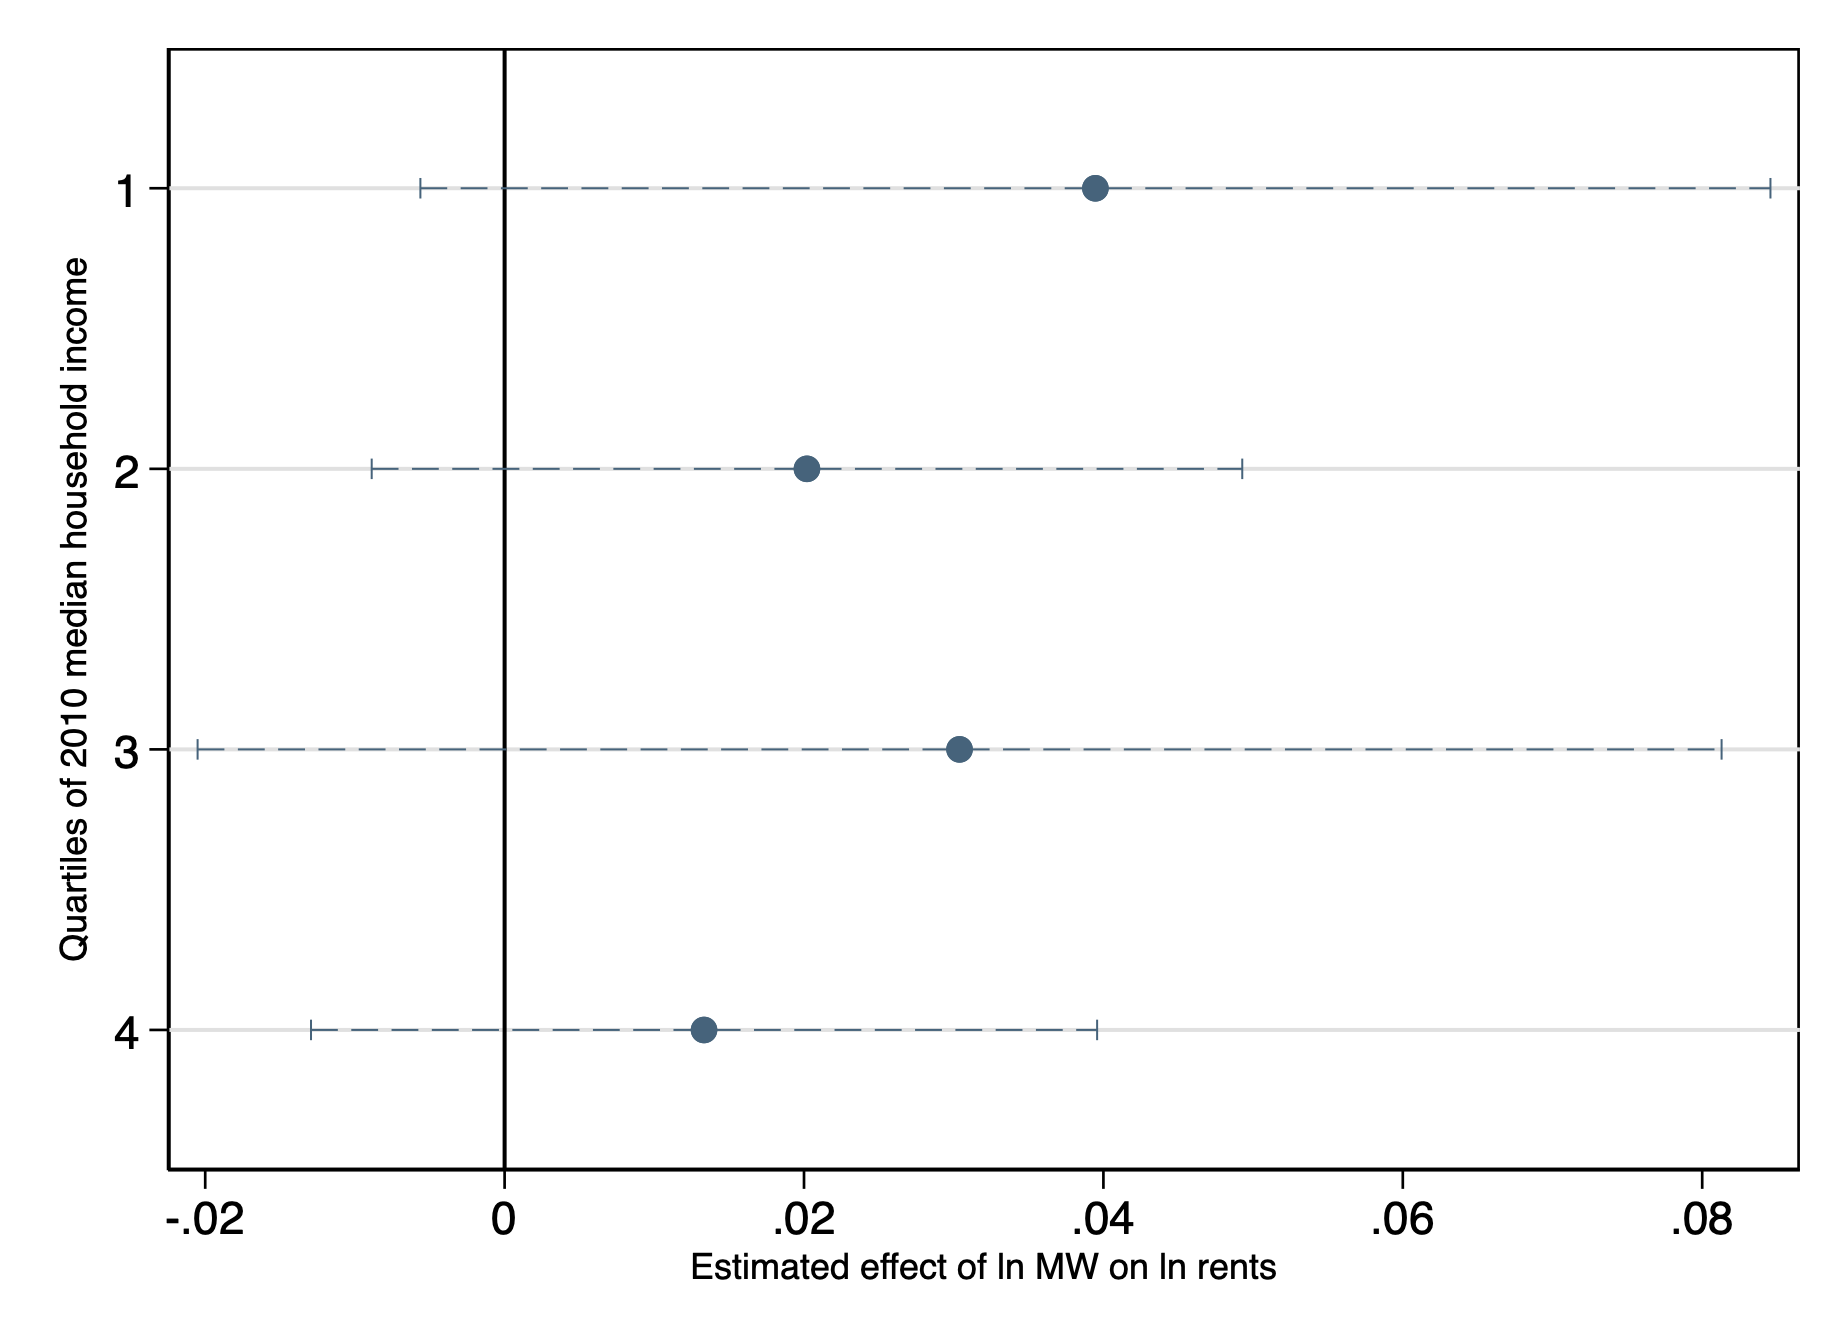
\includegraphics[width=0.75\linewidth]{analysis/first_differences/output/fd_static_heter_med_hhinc20105.png}
        \begin{minipage}{.95\textwidth} \footnotesize
			\vspace{2mm} 
			\textit{Notes}: Results 
		\end{minipage}
    \end{figure}
    
\subsection{Assessing magnitude of the effects}\label{subsec:results/magnitude}


